
\section{Model A - CNN Created From Scratch}
\subsection{Architecture}
Our model architecture is shown in \autoref{fig:ModelAGraph}. 
It consists of a shared trunk with two convolutional layers with 64 3x3 kernels and relu activation followed by a 2x2 maxpooling layer and a batchnorm layer. 
It then has a convolutional layer with 128 3x3 kernels followed by a 2x2 maxpooling layer. 
The output of this trunk is sent to different branches for age and gender prediction. 
The age and gender branches have the same architectureexcept for the number of filters in their final convolutional layers. 
Each branch has two convolutional-maxpooling-batchnorm blocks, the first with 64 3x3 convolutional filters and the second with 128 2x2 filters. 
They are then followed by another convolutional layer of 64 2x2 filters for gender and 128 2x2 filters for age. 
The output of this convolutional layer is then flattened and fed into a 3 layer dense MLP. 
The first layer has 128 node, the second 16 and the final layer is a single node for the output. 
The first and second layers use relu activation and the final layer uses no activation for age prediction and a sigmoid activation for gender prediction.
\begin{notes}
    \\Do we need a full breakdown of the architecture like this?\\
    Given we have the actual graph, think it might be as effective to just include the graph for reference and instead highlight the general arch/approach as you've done below.\\
    We can also include the full architecture output from the summary method in the Appendix if we want to have the breakdown in the report.\\
    Mainly thinking to save on word count.
\end{notes}

\begin{figure}[h!]
    \centering
    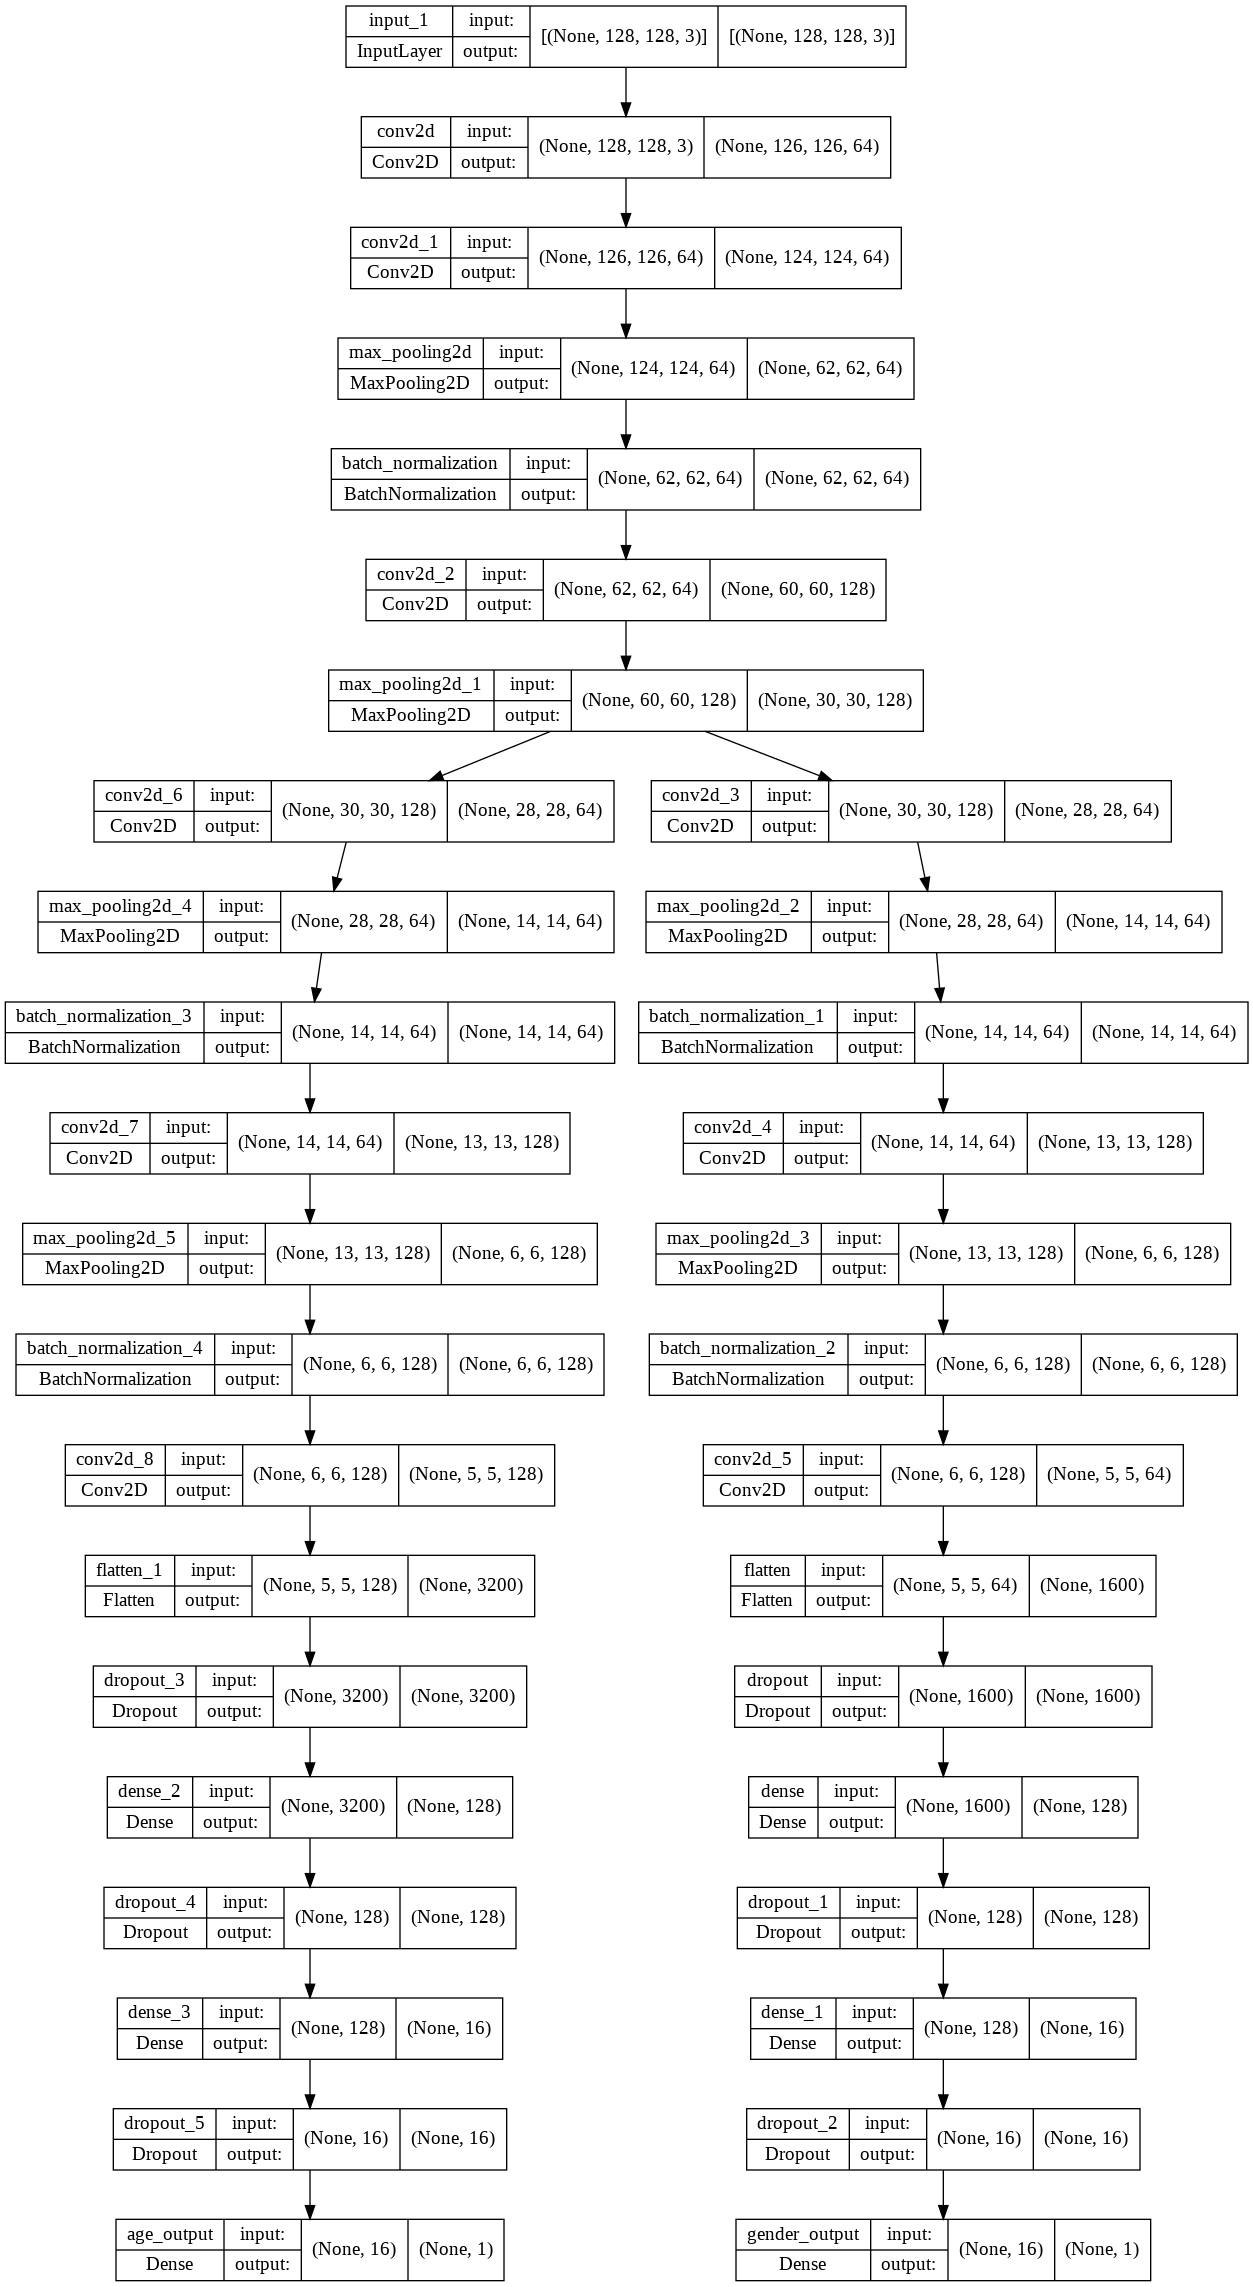
\includegraphics[height=0.95\textheight]{ModelA_Graph.png}
    \caption{The architecture for Model A.}
    \label{fig:ModelAGraph}
\end{figure}

This architecture was chosen because the first layers of a CNN usually extract generic low-level features which are common to many images. 
Therefore using a shared trunk allows the network to use fewer parameters and helps reduce over-fitting.
The branches then allow the model to further extract higher level features specific to age or gender prediction. 
The batchnorm layers help to constrain the gradient delta of weights during training (e.g. preventing some gradients reaching excessive value, large and small). 
The dense layers also employ dropout and L2 regularisation to reduce over-fitting. 

\begin{notes}
    Should we have a subsubsection for the over-fitting prevention?\\
    We already list above as being done for over-fitting, but wondering if having a section would make it more clear?
\end{notes}

\begin{optional}
    \begin{notes}
        A small aside on our previous model to highlight usage of Addition layers and to show improvement seen in new model?\\
        Probably not much here though, as don't want to eat into word count.
    \end{notes}
    \\Prior to arriving at current model, started with overly complex model.\\
    It had X levels of convolutions, batch normalisation and pooling.
    Used addition layers to combat vanishing gradient
    After the convolution layers, two FCN were added, one for each output.
    We also played with performing a conversation to grey scale within the network.
    However training the model (with and without grey scale) did not provide amazing results and faced over-fitting regularly during training (spiky validation)

    One note we were able to draw from the original model was that by having a shared convolution layers we reduced over-fitting.
    We believe this is due to weight adjustment being performed when we had separate convolution layers allowing those layers to fit the training data too well, and by having shared CNN, no weights were able to be adjusted to prioritise a specific feature, and instead be weighted as a compromise to be good for features for both branches.
\end{optional}

\subsection{Training}
The model is trained to minimize a weighted average of losses from each branch. \\
The loss for the gender prediction output is binary cross entropy because it is a binary classification problem and the loss for the age prediction is mean squared error because it is a regression problem. 
Mean squared error was chosen over mean absolute error in order to penalise larger errors more than smaller ones.\\
The average loss is weighted 1:100 towards gender prediction because the average gender losses seen during training were much smaller than the age losses (due to it being a binary problem, and the age loss being a squared value).
This weighting was chosen so the model attempts to balance its training objectives without over-prioritising either age or gender.\\
The model uses the Adam optimizer with a exponentially decaying learning rate.\\
The model is trained for a total of 50 epochs.\\

\begin{optional}
    \subsubsection{Hyper-Parameter Tuning}
    To tune the hyper-parameters we utilized the \verb|keras_tuner|.
    This Keras package allows you to define a set of hyper-parameters for use when building the model. 
    The tuner will build several models, cycling though the different permutations.\\
    It will start with just running a couple of epochs for each permutation, identifying which are the best performing, and then continue training the best parameters for more epochs until the best set is found.\\
    The tuner ignores the training losses, and instead focuses solely on the validation loss, since it's training hyper-params, rather than model weights.\\
    We identified the following hyper-parameters to tune:
    \begin{enumerate}
        \item Greyscale: Whether to apply a greyscale filter to the gender branch, both branches, or neither.
        \item Sigmoid Vs \verb|BinaryCrossEntropy| With logits: whether to use a sigmoid activation on the gender branch or enable logits for the \verb|BinaryCrossEntropy| loss function.
        \item Initial Learning rate
        \item Feature depth of final convolution layer (for both branches)
        \item Dropout rate (for both branches)
        \item Regularisation (for both branches)
    \end{enumerate}
    An output of the tuning can be found in \autoref{appendix:Model_A_Hyper-Parameter_Tuning}

    Once this completed, we rebuilt and trained the model with the tuned hyper-params fixed.\\
    \begin{notes}
        This could be thrown into a table in the appendix if we want to ref we did tuning without wasting space on the specific params?
    \end{notes}
\end{optional}

\subsubsection{Data Preparation}
The model is trained on data from the dataset provided. The data is preprocessed using the Keras \verb|ImageDataGenerator| to effectively increase the size of the dataset and prevent over-fitting. 
The augmentations used are rotation, zoom, and horizontal flipping.\\
To split the dataset into the Training and Validation datasets, the \verb|ImageDataGenerator| was provided 0.2 as the validation split. We then called the \verb|flow_from_dataframe| method on the generator, passing in the dataframe containing the image paths and labels, and provided which dataset should be created, e.g. training or validation.
This created two generators, one for training (utilising 80\% of the dataset), and one for validation (utilising 20\% of the dataset).\\
These generators will then provide augmented versions of the data upon each batch being requested by during the model training.

\subsection{Performance}
Fig \autoref{fig:ModelAPerformanceAge} and \autoref{fig:ModelAPerformanceGender} show the training graphs. 
Our model shows good performance on both age and gender prediction. 
It achieves an accuracy of 93\% for gender prediction and a mean absolute error of 5.6 for age prediction on the training data. 
However it can be seen that the model over-fits slightly and achieves slightly lower performance on the validation data, with an accuracy or 88\% for gender prediction and mean absolute error of 6.8 for age prediction. 
The gender branch can be seen to over-fit to a greater extent than the age branch.

The trace of the final training epoch is below.\\
\begin{verbatim}
Epoch 50/50
125/125 [==============================] 
- 41s 325ms/step 
- loss: 82.5588 
- age_output_loss: 55.1034 
- gender_output_loss: 0.1627 
- age_output_mean_absolute_error: 5.5780 
- gender_output_binary_accuracy: 0.9330 
- val_loss: 131.3783 
- val_age_output_loss: 90.0434 
- val_gender_output_loss: 0.3111 
- val_age_output_mean_absolute_error: 6.8350 
- val_gender_output_binary_accuracy: 0.8821
\end{verbatim}
\begin{notes}
    Throw training output in appendix as it is text?\\
    Can just include gender binary accuracy and age MAE for both training and validation to summarize performance and discuss the graphs?
\end{notes}
\begin{figure}[h]
    \begin{subfigure}{\textwidth}
        \centering
        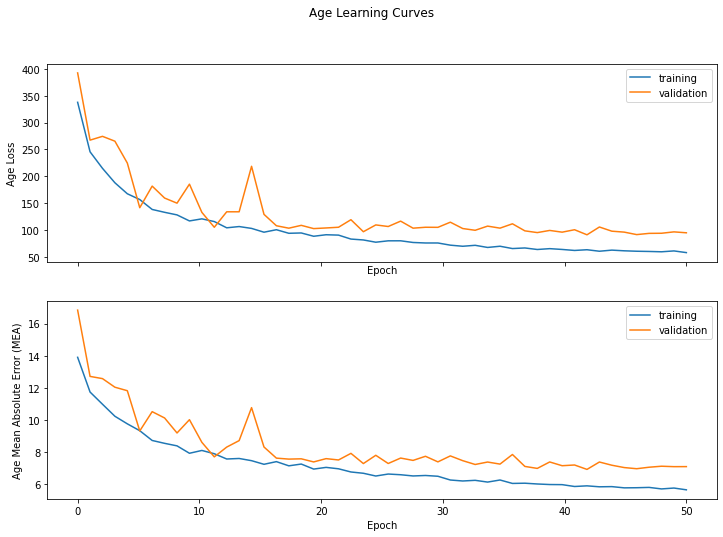
\includegraphics[height=0.45\textheight]{ModelA_AgeLearning_TunedHyperParams.png}
        \caption{\label{fig:ModelAPerformanceAge} The performance on age prediction for our model.}
    \end{subfigure}
    \begin{subfigure}{\textwidth}
        \centering
        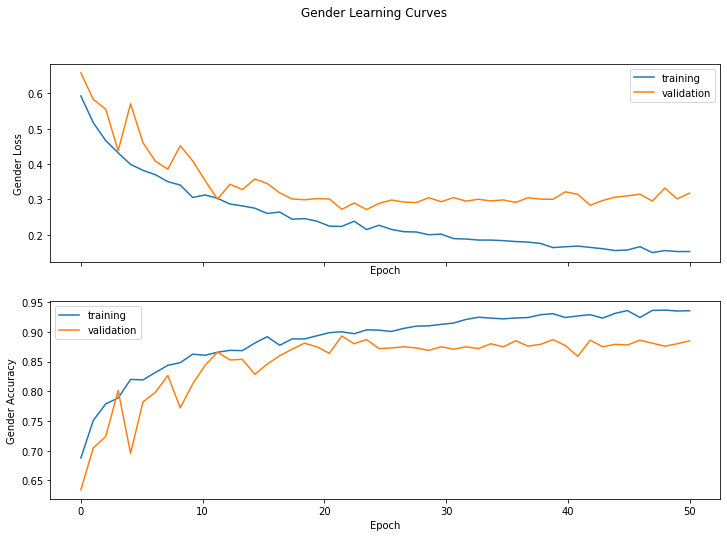
\includegraphics[height=0.45\textheight]{ModelA_GenderLearning_TunedHyperParams.png}
        \caption{\label{fig:ModelAPerformanceGender} The performance on gender prediction for our model.}
    \end{subfigure}
    \label{fig:ModelAPerformance}
    \caption{Learning curves observed training Model A}
\end{figure}
